\section{Methods}
\label{sec:methods}

\subsection{Architecture}
\label{sec:arch}
We propose a method that encodes samples as classifications mapped to
contrastive vectors. This directly constrains a model's representations,
and classifications can natively be used for steering.
Appendix~\ref{app:notation} summarizes our notation.

The model (Figure~\ref{fig:onto-stack}) consists of $l$ $\dictenc$
layers writing into a shared residual accumulator, decoded by a single
linear map. Each layer (Figure~\ref{fig:dictenc}) is composed of a
classifier followed by a dictionary. The classifier splits its input
into $h$ independent \emph{assignments}, each a distribution over one
head's $k$ \emph{entries}, and the dictionary maps each entry to a
representative vector (an \emph{atom}). Each layer writes the
assignment-weighted sum of its atoms to the accumulator; after each
layer the accumulator is decoded and the residual
$\mathbf{x} - \mathrm{dec}(\mathbf{r}_\ell)$ is passed to the next
layer, where $\mathbf{r}_\ell$ accumulates the $\ell$ layers before it.
Deep supervision~\cite{lee2015deeply} constrains every prefix of the
stack to reconstruct the input. Because each layer takes the current
residual as input, components encoded by earlier layers are removed from
the residual passed to later layers, making the code a successive
refinement that is coarse-to-fine in distortion. Unlike in a Tree
SAE~\cite{cao2026}, no later entry is tied to an earlier one, so whether
the code is also coarse-to-fine in concept is an empirical question.

Because entries within a head are mutually exclusive rather than
independent, each dictionary head acts as a contrastive set whose entry
swaps are steering moves. An auxiliary loss term minimizing the
between-head support overlap $\omega$ (Eq.~\eqref{eq:support}) encourages
each head to occupy a disjoint set of dictionary coordinates
(Figure~\ref{fig:head-simplex}), and because each head computes a convex
combination of its atoms, its outputs lie in the simplex spanned by
those atoms (Section~\ref{sec:dict}).

%The mechanism is small enough to quote, excerpted from
%\texttt{dictblock.py} with dtype casts, intervention plumbing, and two
%live no-ops---the identity output activation and the optional per-head
%scaling vector---removed:
%
%\begin{lstlisting}[language=Python]
%def cluster(self, K, temperature=1.0):   # logits -> classifications,
%    return softmax(K / temperature)      # per head, over k entries
%
%def dicts(self):                         # abs() prevents subtractive
%    return jnp.abs(self.weights)         # ontofeatures; (h, k, d)
%
%def fwd(self, P):                        # convex combination per head,
%    return jnp.einsum("...hk,hkd->...d", # summed over heads
%                      P, self.dicts())
%
%def __call__(self, K, temperature=1.0):
%    return self.fwd(self.cluster(K, temperature))
%\end{lstlisting}

\begin{figure}[tp]
\centering
\resizebox{\linewidth}{!}{\begin{tikzpicture}[
    font=\footnotesize,
    >={Stealth[round,length=1.8mm,width=1.6mm]},
    blk/.style={draw, rounded corners=2pt, align=center,
                minimum height=8mm, inner xsep=4pt},
    hook/.style={draw, rounded corners=2pt, densely dashed, align=center,
                 inner sep=3pt, font=\scriptsize, black!55},
    dec/.style={draw, rounded corners=2pt, fill=black!8,
                minimum height=6.5mm, inner xsep=3pt},
    cond/.style={draw, rounded corners=2pt, fill=black!4, align=center,
                 inner sep=2.5pt, font=\scriptsize},
    add/.style={draw, circle, minimum size=4.5mm, inner sep=0pt},
    lab/.style={inner sep=1.5pt, font=\scriptsize},
    sig/.style={->, semithick},
    aux/.style={->, densely dashed, semithick, black!45},
  ]

  %% ---- layer row --------------------------------------------------
  \node[lab] (x)  at (-1.5,0) {$\mathbf{x}\in\mathbb{R}^{d}$};
  \node[blk] (D0) at ( 0.3,0) {$\mathtt{DictEnc}_0$};
  \node[blk] (D1) at ( 4.3,0) {$\mathtt{DictEnc}_1$};
  \node      (Dd) at ( 7.8,0) {$\cdots$};
  \node[blk] (DL) at ( 9.7,0) {$\mathtt{DictEnc}_{l-1}$};

  \draw[sig] (x) -- (D0);

  \node[hook] (noise) at (-1.5,2.6) {$+\,\varepsilon$};
  \draw[aux] (noise) -- (x);

  %% ---- residual accumulator (top rail, y = 2.6) --------------------
  \node[add] (A0) at ( 2.3,2.6) {$+$};
  \node[add] (A1) at ( 6.1,2.6) {$+$};
  \node[add] (AL) at (11.9,2.6) {$+$};

  \node[lab] (R0) at (0.6,2.6) {$\mathbf{r}_0\!=\!\mathbf{0}$};
  \draw[sig]      (R0) -- (A0);
  \draw[sig]      (A0) -- (A1);
  \draw[sig]      (A1) -- (AL);
  \draw[semithick] (AL) -- (12.35,2.6);

  %\node[lab] at (8.9,3.05) {$\mathbf{r}\in\mathbb{R}^{e}$: residual accumulator};

  %% ---- per-layer contributions g_l f'_l (enter from below) ----------
  \draw[sig] (D0.north) -- ++(0,1.1) -| (A0.south);
  \draw[sig] (D1.north) -- ++(0,1.1) -| (A1.south);
  \draw[sig] (DL.north) -- ++(0,1.1) -| (AL.south);
  \node[lab,anchor=west] at (0.38,1.05) {$g_0\mathbf{f}'_0$};
  \node[lab,anchor=west] at (4.38,1.05) {$g_1\mathbf{f}'_1$};
  \node[lab,anchor=west] at (9.78,1.05) {$g_{l-1}\mathbf{f}'_{l-1}$};

  %% ---- shared decoder, one decode per prefix -----------------------
  \node[dec] (Y1) at ( 2.75,-1.9) {$\mathrm{dec}$};
  \node[dec] (Y2) at ( 6.55,-1.9) {$\mathrm{dec}$};
  \node[dec] (YL) at (12.35,-1.9) {$\mathrm{dec}$};

  \draw[sig] ( 2.75,2.6) -- (Y1.north);
  \draw[sig] ( 6.55,2.6) -- (Y2.north);
  \draw[sig] (12.35,2.6) -- (YL.north);
  \fill ( 2.75,2.6) circle (1.1pt);
  \fill ( 6.55,2.6) circle (1.1pt);

  \node[lab,anchor=west] at ( 2.85,1.0) {$\mathbf{r}_1$};
  \node[lab,anchor=west] at ( 6.65,1.0) {$\mathbf{r}_2$};
  \node[lab,anchor=west] at (12.45,1.0) {$\mathbf{r}_{l}$};

  %% ---- deep supervision --------------------------------------------
  \node[lab] (L1) at ( 0.9,-1.9) {$\mathrm{MSE}(\mathbf{x},\hat{\mathbf{x}}_1)$};
  \node[lab] (L2) at ( 4.9,-1.9) {$\mathrm{MSE}(\mathbf{x},\hat{\mathbf{x}}_2)$};
  \node[lab] (LL) at (10.7,-1.9) {$\mathrm{MSE}(\mathbf{x},\hat{\mathbf{x}}_{l})$};
  \draw[aux] (Y1.west) -- (L1);
  \draw[aux] (Y2.west) -- (L2);
  \draw[aux] (YL.west) -- (LL);

  %% ---- residual forwarding ------------------------------------------
  \node[cond] (C1) at (2.75,-3.9)
  {$\mathrm{sg}\,(\mathbf{x}-\hat{\mathbf{x}}_1)$};
  \node[cond] (C2) at (6.55,-3.9)
  {$\mathrm{sg}\,(\mathbf{x}-\hat{\mathbf{x}}_2)$};
  \draw[sig] (Y1) -- node[right,lab]{$\hat{\mathbf{x}}_1$} (C1);
  \draw[sig] (Y2) -- node[right,lab]{$\hat{\mathbf{x}}_2$} (C2);

  \draw[sig] (C1.east) -- node[left,lab,pos=0.72]{$\mathbf{y}_1$} (D1.south);
  \draw[sig] (C2.east) -- node[left,lab,pos=0.72]{$\mathbf{y}_2$} (7.8,-0.5);

  %% ---- model output --------------------------------------------------
  \node[lab] (out) at (12.35,-3.9) {$\hat{\mathbf{x}}$};
  \draw[sig,thick] (YL) -- node[right,lab]{$\hat{\mathbf{x}}_{l}$} (out);

  %% ---- x broadcast to every conditioning step -------------------------
  \draw[aux] (x.south) -- (-1.5,-5.3) -- (2.75,-5.3) -- (C1.south);
  \draw[aux] (2.75,-5.3) -- (6.55,-5.3) -- (C2.south);
  \fill[black!45] (2.75,-5.3) circle (1.1pt);

\end{tikzpicture}

}
\caption[\texttt{Ontologizer} architecture]{\textbf{\texttt{Ontologizer} architecture.}
	An \texttt{Ontologizer} stacks $l$ \texttt{DictEnc} layers, each writing
	its gain-scaled pooled output $g_\ell\mathbf{f}'_\ell$ into a shared
	residual accumulator $\mathbf{r}$. Accumulator states are indexed by the
	number of layers applied: layer $\ell$ receives $\mathbf{r}_\ell$ and the
	residual $\mathbf{y}_\ell = \mathbf{x} - \mathrm{dec}(\mathbf{r}_\ell)$,
	and produces $\mathbf{r}_{\ell+1} = \mathbf{r}_\ell + g_\ell\mathbf{f}'_\ell$.
	A single linear decoder $\mathrm{dec}$ is shared across all layers, and
	every prefix reconstruction is supervised against $\mathbf{x}$ via deep
	supervision. The dashed input-noise hook on $\mathbf{x}$ is disabled in
	every model reported here; Section~\ref{sec:decoder} gives the full
	equations.}
\label{fig:onto-stack}
\end{figure}

\subsubsection{DictEnc}
\label{sec:dictenc}
Each $\dictenc$ consists of a multihead bilinear
classifier~\cite{pirsiavash2009,kim2017} ($\bilinearblock$) with weights
$[\mathsf{W}, \mathsf{V}] \in \mathbb{R}^{2 \times h \times k \times d}$
($d+1$ with the constant coordinate of Eq.~\eqref{eq:y_norm})
and a multihead linear dictionary ($\dictblock$)
with weights $\mathsf{D} \in \mathbb{R}^{h \times k \times e}$.
Layer $\ell$ receives the residual $\mathbf{y}_\ell$ left by earlier
layers ($\mathbf{x}$ itself at layer 0), from which the classifier takes
the normalized shape vector $\mathbf{u}_\ell$ as input
(Eq.~\eqref{eq:y_norm}). Algorithm~\ref{alg:dictenc} specifies the
single-layer training pass, and Algorithm~\ref{alg:ontologizer} specifies
the full stack and loss computation.

\begin{algorithm}[tp]
	\caption{Single-layer $\dictenc$ training pass (\texttt{DictEnc.withStats}).
	When the router is disabled, $\Gamma = \mathbf{1}$ and $\mathrm{L1}_S = 0$;
	when fibers are disabled, the coordinates $\mathsf{C}$ are omitted; and
	when \texttt{resid\_gain} is disabled, the input is not decomposed into
	gain and shape and $g_n = 1$.}
	\label{alg:dictenc}
	\DontPrintSemicolon

	\KwIn{accumulator $R \in \mathbb{R}^{b \times e}$; layer input
		$E \in \mathbb{R}^{b \times d'}$, whose row $n$ is
		$[\mathbf{y}_n;\, \mathbf{1}_{n_{\mathrm{const}}}]$: the varying
		part $\mathbf{y}_n$ (the encoded input at layer 0, the residual
		above) and $n_{\mathrm{const}}$ constant coordinates
		(\texttt{resid\_const})}
	\KwData{bilinear classifier (Eq.~\eqref{eq:bilinearblock}); router
		(\texttt{scaled}); fiber readouts $A_i \in \mathbb{R}^{r \times d'}$;
		$\dictblock$ (Algorithm~\ref{alg:dictblock})}
	\Hyper{logit noise $\sigma_K$; fiber bound $\beta$; the
		$\dictblock$ hyperparameters}
	\KwOut{accumulator $R$; assignments
		$\mathsf{P} \in \mathbb{R}^{b \times h \times k}$; statistics
		row $\boldsymbol{\psi}$ (Eq.~\eqref{eq:stats})}

	\Begin{
		$g_n \leftarrow \mathrm{sg}\big[\lVert \mathbf{y}_n\rVert\big]$;\quad
			$\mathbf{u}_n \leftarrow \big[\mathbf{y}_n/g_n;\,
			\mathbf{1}_{n_{\mathrm{const}}}\big]$
			\tcp*{gain and shape}
		$\mathsf{K}, \mathrm{L1}_K \leftarrow
			\mathrm{classifier}(\mathbf{u}_{1:b})$
			\tcp*{L1 of the gate factor}
		$\mathsf{K} \leftarrow \mathrm{noise}_K(\mathsf{K})$
			\tcp*{Eq.~\eqref{eq:noise_normal} or~\eqref{eq:noise_batchnorm}}
		\eIf{router}{
			$\Gamma, \mathrm{L1}_S \leftarrow \mathrm{router}(\mathbf{u}_{1:b})$;\quad
				$\Gamma \leftarrow \lvert \Gamma \rvert$
				\tcp*{unless \texttt{router\_signed}}
		}{
			$\Gamma \leftarrow \mathbf{1}$;\quad $\mathrm{L1}_S \leftarrow 0$\;
		}
		$\mathbf{c}_{ni} \leftarrow \beta \tanh(A_i \mathbf{u}_n / \beta)$
			\tcp*{fiber coordinates, Eq.~\eqref{eq:fiber}}
		$F', \mathsf{P}, (\mathrm{L1}, H, \mathrm{cossim}_b,
			\mathbb{E}_i\kappa_i, \max_i \kappa_i, \mathrm{KL}_m, \omega)
			\leftarrow \dictblock(\mathsf{K}, \Gamma, \mathsf{C})$\;
		$\mathrm{KL}_{\mathrm{pwak}}, \mathrm{L2}_{\mathrm{pwak}}
			\leftarrow \mathrm{pwak}(\mathsf{P}, \mathbf{u}_{1:b})$
			\tcp*{zero unless enabled}
		$\mathbf{r}_n \leftarrow \mathbf{r}_n + g_n\,\mathbf{f}'_n$
			\tcp*{row $n$ of $R$: the contribution, at the input's gain}
		\Return{$R$, $\mathsf{P}$,
			$\boldsymbol{\psi} = (\mathrm{L1}_K, \mathrm{L1}, H, \mathrm{cossim}_b,
			\mathbb{E}_i\kappa_i, \max_i \kappa_i, \mathrm{KL}_m,
			\mathrm{KL}_{\mathrm{pwak}}, \mathrm{L2}_{\mathrm{pwak}},
			\mathrm{L1}_S, \omega)$}\;
	}
\end{algorithm}


\begin{figure}[tp]
\centering
\resizebox{\linewidth}{!}{\begin{tikzpicture}[
    font=\footnotesize,
    >={Stealth[round,length=1.8mm,width=1.6mm]},
    blk/.style={draw, rounded corners=2pt, align=center,
                minimum height=8mm, inner xsep=4pt},
    hook/.style={draw, rounded corners=2pt, densely dashed, align=center,
                 inner sep=3pt, font=\scriptsize, black!55},
    lab/.style={inner sep=1.5pt, font=\scriptsize, align=center},
    sig/.style={->, semithick, align=center},
    aux/.style={->, densely dashed, semithick, black!45},
  ]

  %% ---- main chain ----------------------------------------------------
  \node[lab] (E)  at (-0.6,0) {$\mathbf{u}$};
  \node[blk] (CL) at ( 1.2,0) {$\bilinearblock^{d \to h \times k}$};
  \node[blk] (SM) at ( 4.9,0) {$\mathrm{softmax}_k(\cdot/t)$};
  \node[blk] (DB) at ( 9.4,0) {$\dictblock^{h \times k \to h \times e}$};
  \node[blk] (SU) at (12.3,0) {$\sum^{h}_{i=1}$};
  \node[lab] (F)  at (13.6,0) {$\mathbf{f}'$\\ pooled\\ features};

  \draw[sig] (E)  -- (CL);
  \draw[sig] (CL) -- node[below,lab]{$K$\\ logits}   (SM);
  \draw[sig] (SM) -- node[below,lab]{$P$\\ classifications}   (DB);
  \draw[sig] (DB) -- node[below,lab]{$F$\\ features} (SU);
  \draw[sig] (SU) -- (F);

  %% ---- training-time hooks and the intervention interface (above) ----
  \node[hook] (nk) at (3.0,1.5) {$+\,\varepsilon_K$,\ winner dropout};
  \node[hook] (iv) at (7.0,2.3) {\texttt{DictIntervention}\\
                                 set / add / sub / ablate / scale};
  \node[hook] (nf) at (11.4,1.5) {$+\,\varepsilon_F$};
  \draw[aux] (nk) -- (3.0,0.20);
  \draw[aux] (iv) -- (7.0,0.20);
  \draw[aux] (nf) -- (11.4,0.20);

  %% ---- where each regulariser attaches (below) -----------------------
  \node[hook] (lp) at (4.9,-1.8)
    {$H$\quad $\mathrm{KL}_m$\quad $\mathrm{cossim}_b$};
  \node[hook] (lf) at (9.4,-1.8)
    {$\mathrm{L1}$\quad $\omega$};
  \draw[aux] (SM.south) -- (lp);
  \draw[aux] (DB.south) -- (lf);

\end{tikzpicture}

}
\caption[\texttt{DictEnc} architecture]{\textbf{\texttt{DictEnc} architecture.}
	A multihead bilinear classifier maps the normalized shape vector
	$\mathbf{u}$ to logits $K$; assignments $P = \mathrm{softmax}_k(K/t)$
	(or their straight-through argmax) weight the dictionary atoms to form
	per-head features $F$, which are summed across heads into pooled features
	$\mathbf{f}'$. Dashed boxes above the main path represent training
	perturbations and causal interventions; dashed boxes below represent
	summary statistics that serve as tunable auxiliary loss terms
	(Sections~\ref{sec:bilinear}--\ref{sec:dict}).}
\label{fig:dictenc}
\end{figure}

\subsubsection{Classifier}
\label{sec:bilinear}
For a generic input $\mathbf{x} \in \mathbb{R}^d$ (in layer $\ell$, the
normalized shape vector $\mathbf{u}_\ell \in \mathbb{R}^{d+1}$), the
multihead bilinear classifier $\bilinearblock$ computes logits
$K \in \mathbb{R}^{h \times k}$ via
\begin{equation}
	\bilinearblock([\mathsf{W},\mathsf{V}],\mathbf{x}) :=
	\left(\sum^{d}_{q=1}W_{\cdot\cdot q}\,x_q\right)
	 \odot \left(\sum^{d}_{q=1}V_{\cdot\cdot q}\,x_q\right).
	 \label{eq:bilinearblock}
\end{equation}
Each logit is a quadratic form in $\mathbf{x}$, the low-rank form of
bilinear classifiers~\cite{pirsiavash2009,kim2017}, so the classifier
admits closed-form eigendecomposition in the manner of bilinear
MLPs~\cite{pearce2025}. During training, optional Gaussian noise
$\varepsilon_K$ is added to the logits (Section~\ref{sec:noise}), and
winner dropout sets each head's maximum logit to $-\infty$ with
probability $p_{\mathrm{drop}}$.

\subsubsection{Assignments and selection}
\label{sec:labels}
Soft assignments are given by $P = \mathrm{softmax}_{k}(K/t)$, where the
temperature hyperparameter $t$ is annealed during training to sharpen the
distributions (schedules in Appendix~\ref{app:configs}). Under the
\emph{straight-through} selection rule (\texttt{ste}), the forward pass
selects the one-hot argmax while the backward pass uses
$\mathrm{softmax}_k(K/t)$ as a surrogate gradient~\cite{bengio2013,jang2017};
intermediate \texttt{top}$k_{\mathrm{sel}}$ rules apply a softmax to each
head's top $k_{\mathrm{sel}}$ logits and zero the remainder. Causal
interventions act directly on the assignments $P$.

From $P$ we compute three assignment statistics. The first is per-sample
entropy $H$, measured in bits so that each head saturates at $\log_2 k$
bits ($5$ bits at $k{=}32$),
\begin{equation}
	\mathrm{entropy}_k(\mathbf{p}) :=
	-\sum^{k}_{j=1}p_{j}\log_2 p_{j},
	\qquad
	H := \mathbb{E}_{n}\,\mathbb{E}_{i}\!\left[
	\mathrm{entropy}_k(\mathbf{p}_{ni})\right].
	\label{eq:entropy}
\end{equation}
The second is between-sample similarity $\mathrm{cossim}_b$, the mean
absolute cosine similarity of the concatenated per-head features over all
ordered pairs of samples,
\begin{equation}
	\mathrm{cossim}_b :=
	\mathbb{E}_{n,n'}\big\lvert
	\cos\angle(\mathbf{f}_{n}, \mathbf{f}_{n'})
	\big\rvert,
	\qquad
	\langle \mathbf{f}_{n}, \mathbf{f}_{n'}\rangle
	= \sum^{h}_{i=1}\gamma_{ni}\gamma_{n'i}\,
	\mathbf{p}_{ni}^{\top}G_{i}\,\mathbf{p}_{n'i},
	\label{eq:cossim_b}
\end{equation}
where $\mathbf{f}_{ni} := \mathsf{F}_{ni\cdot} \in \mathbb{R}^{e}$ is
head $i$'s feature vector on sample $n$,
$\mathbf{f}_n = \map_{i=1}^{h}\mathbf{f}_{ni}$ is their concatenation,
$\gamma_{ni}$ is head $i$'s router scale on sample $n$ ($1$ without a
router; Section~\ref{sec:router-fiber}), and
$G_i = \lvert D_{i}\rvert \lvert D_{i}\rvert^{\top} \in \mathbb{R}^{k \times k}$
is head $i$'s dictionary Gram matrix, with
$D_i := \mathsf{D}_{i\cdot\cdot} \in \mathbb{R}^{k \times e}$ ($G_i =
D_i D_i^\top$ when the dictionary is signed). Evaluating
Eq.~\eqref{eq:cossim_b} in entry space through $G_i$ rather than
materializing $\mathsf{F}$ yields identical values and gradients while
reducing the cost from $\mathcal{O}(b^2he)$ to
$\mathcal{O}(hk^2e + b^2hk)$. Finally, $\mathrm{KL}_m$ is the divergence
of the batch-mean assignment from uniform, in bits, averaged across
heads:
\begin{equation}
	\mathrm{KL}_m := \mathbb{E}_{i}\!\left[\log_2 k -
	\mathrm{entropy}_k\!\left(\bar{\mathbf{p}}_i\right)\right],
	\qquad
	\bar{\mathbf{p}}_i := \mathbb{E}_{n}\,[\mathbf{p}_{ni}].
	\label{eq:KL}
\end{equation}
In practice an explicit penalty on $H$ is unnecessary, because minimizing
$\mathrm{cossim}_b$ also reduces per-sample entropy. The batch-mean
uniformity term $\mathrm{KL}_m$ anchors each head's mean assignment
$\bar{\mathbf{p}}_i$ to the uniform distribution: this keeps all $k$
entries active---a head that collapses onto a single entry incurs the
full $\log_2 k$-bit penalty---and encourages a uniform assignment
$\mathbf{p}_{ni}$ to represent a maximally generic feature vector.

\subsubsection{Dictionary}
\label{sec:dict}
A $\dictblock$ maps assignments $P \in \mathbb{R}^{h \times k}$ to
per-head features $F \in \mathbb{R}^{h \times e}$, whose row
$\mathbf{f}_i$ is head $i$'s output:
\begin{equation}
	\dictblock(\mathsf{D},P)_{i\cdot} = \mathbf{f}_i :=
	\sum^{k}_{j=1} p_{ij}\,\mathbf{a}_{ij},
	\qquad
	\mathbf{a}_{ij} := \lvert \mathsf{D}_{ij\cdot}\rvert,
	\label{eq:dictblock}
\end{equation}
where the atom $\mathbf{a}_{ij}$ is the elementwise absolute value of
head $i$'s dictionary vector for entry $j$ ($\mathsf{D}_{ij\cdot}$ itself
when the dictionary is signed). Because the atoms are non-negative and
$p_{ij} \in [0,1]$, features are strictly additive; because each head's
assignment sums to one, $\mathbf{f}_i$ lies in the simplex whose vertices
are the head's atoms (Figure~\ref{fig:head-simplex}), matching the
geometry that Park et al.~\cite{park2025} derive for representations of
categorical concepts, in which entries represent mutually exclusive
alternatives rather than independently firing features. This lookup takes
the form of attention over a learned per-head memory---a softmax over
input-dependent entry scores weighting the atoms as
values~\cite{bahdanau2015,luong2015,vaswani2017}---and, when paired with
a linear classifier, coincides with a single update of a modern Hopfield
layer at inverse temperature $1/t$~\cite{ramsauer2021}.
Algorithm~\ref{alg:dictblock} details the full training pass, including
the regularizing perturbations and auxiliary statistics computed
alongside the lookup.

\begin{algorithm}[tp]
	\caption{$\dictblock$ training pass (\texttt{DictBlock.withStats}). At
	inference time, the four stochastic steps (revival, winner dropout, head
	dropout, and fiber dropout) and feature noise are omitted. Every
	statistic is stop-gradiented unless its corresponding loss term is
	enabled.}
	\label{alg:dictblock}
	\DontPrintSemicolon
	\footnotesize

	\KwIn{logits $\mathsf{K} \in \mathbb{R}^{b \times h \times k}$;
		router scales $\Gamma \in \mathbb{R}_{\ge 0}^{b \times h}$ (all ones
		without a router); fiber coordinates
		$\mathsf{C} \in \mathbb{R}^{b \times h \times r}$ (none without
		fibers)}
	\KwData{dictionary $\mathsf{D} \in \mathbb{R}^{h \times k \times e}$;
		fiber bases $U_{ij} \in \mathbb{R}^{e \times r}$}
	\Hyper{temperature $t$; feature noise $\sigma_F$; winner dropout
		$p_{\mathrm{drop}}$; revival rate $p_{\mathrm{rev}}$ and threshold
		$\tau_{\mathrm{rev}}$; head dropout $p_{\mathrm{head}}$; fiber dropout
		$p_{\mathrm{fib}}$; entries kept per head $k_{\mathrm{sel}}$
		($1$ under \texttt{ste}/\texttt{argmax}, $k$ under softmax, and
		the rule's own value under \texttt{top}$k_{\mathrm{sel}}$, e.g.\ 4
		for \texttt{top4})}
	\KwOut{pooled features $F' \in \mathbb{R}^{b \times e}$; assignments
		$\mathsf{P} \in \mathbb{R}^{b \times h \times k}$; statistics
		$(\mathrm{L1}, H, \mathrm{cossim}_b, \mathbb{E}_i\kappa_i,
		\max_i \kappa_i, \mathrm{KL}_m, \omega)$}

	\Begin{
		$\mathbf{a}_{ij} \leftarrow \lvert \mathsf{D}_{ij\cdot} \rvert$
			\tcp*{atoms; $\mathsf{D}_{ij\cdot}$ itself if signed}
		\If(\tcp*[f]{revive starved entries}){$k_{\mathrm{sel}} < k$}{
			$\mathrm{use}_{ij} \leftarrow$ share of rows on which entry $j$
				is among head $i$'s top $k_{\mathrm{sel}}$ logits\;
			\ForEach{$(n,i)$ with probability $p_{\mathrm{rev}}$}{
				draw $j$ uniformly from $\{j : \mathrm{use}_{ij} <
					\tau_{\mathrm{rev}}\,k_{\mathrm{sel}}/k\}$, if any\;
				raise entry $j$'s logit on row $n$ to head $i$'s maximum
					\tcp*{tie the leader}
			}
		}
		each $(n,i)$: $\max_j [\mathsf{K}]_{nij} \leftarrow -\infty$ with probability
			$p_{\mathrm{drop}}$ \tcp*{winner dropout}
		$\mathsf{P} \leftarrow \mathrm{select}_k(\mathsf{K}/t)$
			\tcp*{softmax, \texttt{top}$k_{\mathrm{sel}}$ or straight-through}
		$H \leftarrow \mathbb{E}_{n,i}\,\mathrm{entropy}_k(\mathbf{p}_{ni})$
			\tcp*{Eq.~\eqref{eq:entropy}}
		$\bar{\mathbf{p}}_i \leftarrow \mathbb{E}_n\,\mathbf{p}_{ni}$;\quad
			$\mathbf{o}_i \leftarrow \mathrm{sg}[\bar{\mathbf{p}}_i]$
			\tcp*{usage; head origin}
		\ForEach(\tcp*[f]{head dropout}){$(n,i)$}{
			$\mathbf{p}'_{ni} \leftarrow \mathbf{o}_i$ with
				probability $p_{\mathrm{head}}$, else
				$\mathbf{o}_i + (\mathbf{p}_{ni} - \mathbf{o}_i)
				/ (1 - p_{\mathrm{head}})$\;
		}
		each $(n,i)$: $\mathbf{c}_{ni} \leftarrow \mathbf{0}$ with
			probability $p_{\mathrm{fib}}$ \tcp*{fiber dropout}
		$\mathbf{f}_{ni} \leftarrow \gamma_{ni} \sum_{j} p'_{nij}\,
			\mathbf{a}_{ij}$ \tcp*{Eq.~\eqref{eq:dictblock}; interventions act
			on $\mathbf{p}'$}
		$\tilde{\mathsf{F}} \leftarrow \mathrm{noise}_{\mathrm{featvar}}
			(\mathsf{F})$ \tcp*{Eq.~\eqref{eq:noise_featvar}}
		$\mathrm{cossim}_b \leftarrow \mathbb{E}_{n,n'}
			\lvert\cos\angle(\mathbf{f}_n, \mathbf{f}_{n'})\rvert$, with
			$\mathbf{f}$ built from $\mathsf{P}$, not $\mathsf{P}'$
			\tcp*{Eq.~\eqref{eq:cossim_b}, through the Grams}
		$\kappa_i \leftarrow \mathbb{E}_{j \ne j'}
			\cos\angle(\mathbf{a}_{ij}, \mathbf{a}_{ij'})$
			\tcp*{within-head atom cosine}
		$\mathrm{KL}_m \leftarrow \mathbb{E}_i \left[\log_2 k -
			\mathrm{entropy}_k(\bar{\mathbf{p}}_i)\right]$
			\tcp*{Eq.~\eqref{eq:KL}}
		$\boldsymbol{\pi}_i \leftarrow \sum_j \bar{p}_{ij}\,
			\lvert\mathbf{a}_{ij}\rvert$;\quad
			$\omega \leftarrow \mathbb{E}_{i \ne i'}
			\cos\angle(\boldsymbol{\pi}_i, \boldsymbol{\pi}_{i'})$
			\tcp*{support overlap}
		$\mathrm{L1} \leftarrow \mathbb{E}_n \sum_i
			\lVert \tilde{\mathbf{f}}_{ni} \rVert_1$\;
		$\mathbf{f}'_n \leftarrow \sum_i \tilde{\mathbf{f}}_{ni}$
			\tcp*{concatenated, not summed, under $\mathtt{ConcatDictBlock}$}
		\If(\tcp*[f]{Eq.~\eqref{eq:fiber}, then any norm cap}){fibers}{
			$\mathbf{f}'_n \leftarrow \mathbf{f}'_n + \sum_i \gamma_{ni}
				\sum_j p'_{nij}\,U_{ij}\,\mathbf{c}_{ni}$\;
		}
		\Return{$F'$, $\mathsf{P}$,
			$(\mathrm{L1}, H, \mathrm{cossim}_b, \mathbb{E}_i\kappa_i,
			\max_i \kappa_i, \mathrm{KL}_m, \omega)$}\;
	}
\end{algorithm}


From the assignments and atoms we compute the between-head support
overlap $\omega$, defined as the mean cosine similarity across ordered
pairs of distinct heads between their usage-weighted coordinate profiles
$\boldsymbol{\pi}_i$:
\begin{equation}
	\boldsymbol{\pi}_i := \sum^{k}_{j=1} \bar{p}_{ij}\,
	\lvert \mathbf{a}_{ij}\rvert,
	\qquad
	\omega := \mathbb{E}_{i \neq i'}\,
	\frac{\langle \boldsymbol{\pi}_i, \boldsymbol{\pi}_{i'}\rangle}
	     {\lVert \boldsymbol{\pi}_i\rVert \lVert \boldsymbol{\pi}_{i'}\rVert},
	\label{eq:support}
\end{equation}
with $\bar{\mathbf{p}}_i$ the batch-mean assignment of
Eq.~\eqref{eq:KL}. The overlap $\omega$ vanishes if and only if no two
heads share an active coordinate of the dictionary space, and equals one
when all heads weight the coordinates in identical proportions
(Section~\ref{sec:disjoint}). Computing $\omega$ requires
$\mathcal{O}(hke + h^2e)$ operations, independent of the batch size $b$;
weighting by $\bar{\mathbf{p}}_i$ excludes dead entries from the profile
and provides a gradient path to the classifier. Figure~\ref{fig:anatomy}
illustrates the assignments, atoms, and both cosine statistics for a
single trained head.

After feature noise $\varepsilon_F$ is added to form
$\tilde{\mathsf{F}} := \mathsf{F} + \varepsilon_F$
(Section~\ref{sec:noise}), we also compute the feature sparsity penalty
\begin{equation}
	\mathrm{L1}(\tilde{\mathsf{F}}) :=
	\frac{1}{b}\sum^{b}_{n=1}\sum^{h}_{i=1}\sum^{e}_{q=1}
	\lvert \tilde{f}_{niq}\rvert.
	\label{eq:L1}
\end{equation}
Because $\mathrm{L1}$ averages each sample's L1 norm across the
batch, it is invariant to $b$ and scales with $h$ and $e$, so its loss
weight is correspondingly small; although $\mathrm{L1}$ decreases under
$\mathrm{MSE}$ training alone, penalizing it explicitly accelerates
convergence.

\begin{figure}[tp]
\centering
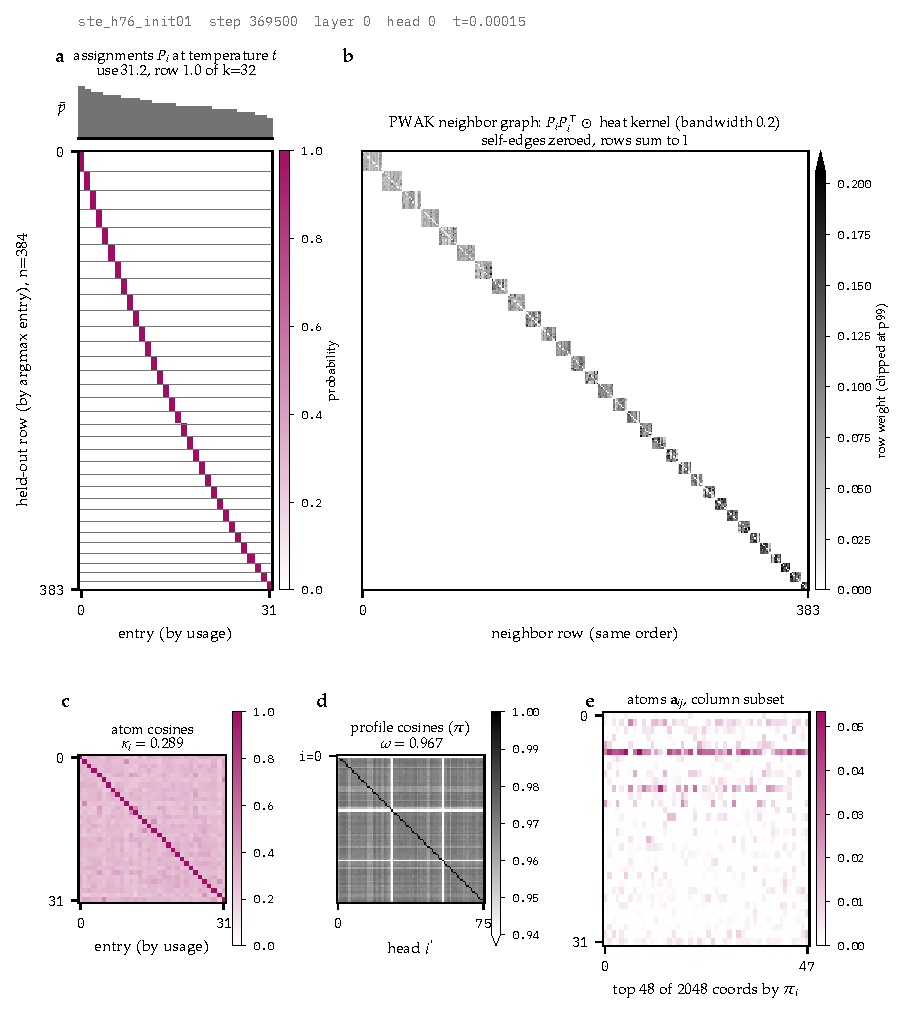
\includegraphics[width=0.85\linewidth]{figures/fig-anatomy.pdf}
\caption[One trained head, block by block]{\textbf{One trained head,
	block by block.} Head $i{=}0$ of layer 0 in \texttt{ste\_h76\_init01}
	(step 369{,}500, $t{=}0.00015$) on $n{=}384$ held-out rows; one seed.
	(a) Assignments $P_i$, with rows sorted by winning entry and entries by
	mean usage $\bar{p}_{ij}$ (bars). ``Use'' is the effective entry count
	across rows, $2^{\mathrm{entropy}_k(\bar{\mathbf{p}}_i)}$, and ``row''
	within a row, $2$ raised to the mean per-row entropy ($31.2$ and $1.0$
	of $k{=}32$, a hard code using nearly every entry). (b) The neighbor
	graph for $\mathrm{KL}_{\mathrm{pwak}}$ and $\mathrm{L2}_{\mathrm{pwak}}$
	(Eq.~\eqref{eq:stats}) in the same row order: the elementwise product of
	$P_iP_i^\top$ and the shape heat kernel
	$\exp((\langle\mathbf{u}_n,\mathbf{u}_{n'}\rangle - 1)/0.2)$ (excluding
	the constant coordinate), with self-edges zeroed and rows normalized to
	unit sum. Hard selection makes this matrix block-diagonal by cell;
	because neither PWAK term was active in training, it reflects the
	induced graph alone. (c) Pairwise cosines among head $i$'s atoms
	(off-diagonal mean $\kappa_i = 0.289$). (d) Pairwise cosines among head
	coordinate profiles $\boldsymbol{\pi}$ (Eq.~\eqref{eq:support}) using
	the $n$-row mean $\bar{\mathbf{p}}$ (off-diagonal mean $\omega = 0.967$,
	head $i$ outlined). (e) Head $i$'s atoms on the 48 of $e{=}2048$
	coordinates where $\boldsymbol{\pi}_i$ is largest (a column subset, not
	a projection). Each panel sets zero to white, except (d), whose scale
	starts at the 5th percentile of off-diagonal cosines because $\omega$ is
	near $1$. Figure~\ref{fig:anatomy-softmax} shows the softmax counterpart.}
\label{fig:anatomy}
\end{figure}

\paragraph{Disjoint support}
\label{sec:disjoint}
Between heads, orthogonality of non-negative features acts as a
support-partition condition rather than a rotation constraint. Every
feature vector $\mathbf{f}_{ni}$ lies in the non-negative orthant of
$\mathbb{R}^e$, since $\lvert \mathsf{D} \rvert \geq 0$ and $P \geq 0$.
For non-negative vectors $\mathbf{v}, \mathbf{v}'$, the inner product
$\langle \mathbf{v},\mathbf{v}'\rangle = \sum_q v_q v'_q$ is a sum of
non-negative terms and therefore vanishes if and only if every term
vanishes:
\begin{equation}
	\langle \mathbf{v},\mathbf{v}'\rangle = 0
	\iff
	\mathrm{supp}(\mathbf{v}) \cap \mathrm{supp}(\mathbf{v}') = \emptyset.
	\label{eq:disjoint}
\end{equation}
Non-negative sparse PCA and orthogonal non-negative matrix factorization
rely on the same equivalence: orthonormal non-negative components
partition the coordinates among themselves~\cite{zass2006,asteris2015onmf}.
Signed vectors admit no such implication, because orthogonality can arise
through cancellation even when two vectors share identical support; a
penalty on inner products between sets of signed atoms, such as the
incoherence penalty that Ramirez et al.~\cite{ramirez2010} apply across
per-class dictionaries, can therefore be satisfied without coordinate
disjointness. The support overlap $\omega$ of Eq.~\eqref{eq:support}
avoids this ambiguity by taking elementwise absolute values of the atoms,
whose inner products vanish if and only if their supports are disjoint
regardless of atom signs, and by aggregating clean atoms weighted by
$\bar{\mathbf{p}}_i$ rather than noisy features $\tilde{\mathsf{F}}$,
whose additive noise can drive coordinates negative.

Under softmax selection, this condition constrains the dictionary weights
directly rather than merely individual sample activations. Because
softmax assignments satisfy $p_{nij} > 0$ for every entry, expanding
Eq.~\eqref{eq:dictblock} yields
\begin{equation}
	\langle \mathbf{f}_{ni},\mathbf{f}_{ni'}\rangle =
	\sum^{k}_{j=1}\sum^{k}_{j'=1} p_{nij}\,p_{ni'j'}
	\left\langle \mathbf{a}_{ij}, \mathbf{a}_{i'j'} \right\rangle,
	\label{eq:cross_head}
\end{equation}
a strictly positive linear combination of all $k^2$ cross-head atom inner
products. Consequently, if heads $i$ and $i'$ are orthogonal on even a
single sample, $\langle \mathbf{a}_{ij}, \mathbf{a}_{i'j'}\rangle = 0$
must hold for every atom pair $(j,j')$, partitioning the coordinates of
$\mathsf{D}$ across heads for all inputs rather than only on the training
distribution. This provides the weight-level guarantee required for a
static reading of the dictionary, which no signed-feature inner-product
penalty can enforce. Dimensionally, such a partition is well within
capacity: in the softmax configuration (Table~\ref{tab:cfg-softmax}),
dividing $e{=}2048$ coordinates among $h{=}32$ heads allocates 64
coordinates per head to represent $k{=}32$ atoms, which need not have
disjoint supports within a head. Accommodating between-head disjointness
is the primary motivation for choosing an overcomplete dictionary width
$e > d$.

Two distinct forms of orthogonality are therefore at play, only the
between-head one being architectural: disjoint support assigns each head
its own coordinate block, whereas \emph{within} a head the $k$ atoms act
as contrastive alternatives spread across that block
(Figure~\ref{fig:head-simplex}; Section~\ref{sec:prelim-orth}). When
heads are summed, neither property is guaranteed at convergence because
$\omega$ acts only as a soft penalty; similarly, in non-negative matrix
factorization, soft overlap penalties reduce coordinate sharing without
yielding an exact partition, which instead requires hard coordinate
assignment~\cite{zass2006,pompili2014,asteris2015onmf,charikar2021}.
Empirically, summed models exhibit strong within-head contrast at
convergence while failing to partition coordinates between heads
(Appendix~\ref{sec:support}). In the concatenated-head variant
($\mathtt{ConcatDictBlock}$), by contrast, each head writes to a
dedicated coordinate slice by construction and $\omega$ is identically
zero (Section~\ref{sec:geom}, Appendix~\ref{sec:concatgeom}, and
Section~\ref{sec:gpt2hard}).

Finally, the noisy per-head features $\tilde{\mathbf{f}}_i$ are summed
across heads (or concatenated across slices under
$\mathtt{ConcatDictBlock}$) to form the pooled layer output
$\mathbf{f}' \in \mathbb{R}^{e}$ written to the accumulator $\mathbf{r}$:
\begin{equation}
	\mathbf{f}' = \sum^{h}_{i=1}\tilde{\mathbf{f}}_{i}.
	\label{eq:pool}
\end{equation}

\begin{figure}[tp]
\centering
\begin{tikzpicture}[
    font=\footnotesize,
    >={Stealth[round,length=1.8mm,width=1.6mm]},
    lab/.style={inner sep=1.5pt, font=\scriptsize},
  ]
  %% ---- head i --------------------------------------------------------
  \fill[black!8]   (0,0) -- (2.4,0) -- (1.2,2.0) -- cycle;
  \draw[semithick] (0,0) -- (2.4,0) -- (1.2,2.0) -- cycle;
  \fill (0,0)     circle (1.5pt) node[below,lab]{$\mathbf{a}_{i1}$};
  \fill (2.4,0)   circle (1.5pt) node[below,lab]{$\mathbf{a}_{i2}$};
  \fill (1.2,2.0) circle (1.5pt) node[above,lab]{$\mathbf{a}_{i3}$};
  \fill (1.05,0.72) circle (1.7pt) node[left,lab]{$\mathbf{f}_i$};

  %% ---- head i' ------------------------------------------------------
  \fill[black!8]   (5.0,0) -- (7.4,0) -- (6.2,2.0) -- cycle;
  \draw[semithick] (5.0,0) -- (7.4,0) -- (6.2,2.0) -- cycle;
  \fill (5.0,0)   circle (1.5pt) node[below,lab]{$\mathbf{a}_{i'1}$};
  \fill (7.4,0)   circle (1.5pt) node[below,lab]{$\mathbf{a}_{i'2}$};
  \fill (6.2,2.0) circle (1.5pt) node[above,lab]{$\mathbf{a}_{i'3}$};
  \fill (6.55,0.60) circle (1.7pt) node[right,lab]{$\mathbf{f}_{i'}$};

  \draw[<->, densely dashed, semithick, black!55] (1.35,0.71) -- (6.30,0.61);
  \node[lab] at (3.85,1.35)
    {$\omega$ penalizes heads $i$, $i'$ sharing coordinates};

  \node[lab, anchor=north, align=center] at (3.7,-0.9)
  {$\mathbf{f}'=\sum^h_{i=1} \mathbf{f}_i$,\qquad
  $\mathbf{f}_i=\sum^k_{j=1} p_{ij}\,\mathbf{a}_{ij}$,\qquad $\sum^k_{j=1} p_{ij}=1$};
\end{tikzpicture}


\caption[Per-head geometry]{\texttt{DictBlock} \textbf{head geometry} for $h{=}2$, $k{=}3$.
	Each head's output $\mathbf{f}_i$ lies in the simplex spanned by its
	atoms $\mathbf{a}_{ij}$ (the rows of $\lvert D_i\rvert$), at the convex
	combination selected by its assignment $\mathbf{p}_i$. Because
	$\lvert\mathsf{D}\rvert \geq 0$ and $P \geq 0$, features are
	non-negative and $\cos\angle(\mathbf{f}_i, \mathbf{f}_{i'}) \in [0,1]$;
	driving the support overlap $\omega$ toward zero encourages heads to
	occupy disjoint coordinates of $\mathbb{R}^e$
	(Section~\ref{sec:disjoint}).}
\label{fig:head-simplex}
\end{figure}

\subsubsection{Decoder}
\label{sec:decoder}
Each layer's pooled output $\mathbf{f}'_\ell$ is scaled by its input's
gain $g_\ell$ and added to the residual accumulator $\mathbf{r}$, whose
state after $\ell$ layers is
\begin{equation}
	\mathbf{r}_\ell = \sum_{\ell'=0}^{\ell-1} g_{\ell'}\,\mathbf{f}'_{\ell'},
	\qquad
	g_\ell := \mathrm{sg}\!\left[\mathrm{L2}(\mathbf{y}_\ell)\right].
	\label{eq:accum}
\end{equation}
When gain scaling (\texttt{resid\_gain}) is enabled, each layer
classifies only the direction of its input while $g_\ell$ restores the
residual's norm; otherwise $g_\ell = 1$. At $\ell = 0$ the empty sum
gives $\mathbf{r}_0 = \mathbf{0}$, so layer 0 receives the encoded input
$\mathbf{y}_0 = \mathbf{x}$ directly, with $g_0 = 1$ identically on
unit-norm SONAR embeddings.

A single unbiased linear decoder $\mathrm{dec}$ with weights
$W_{\mathrm{dec}} \in \mathbb{R}^{d \times e}$, shared across all
$\dictenc_\ell$ layers (or replaced by the identity in direct-atom
variants, where $e = d$), projects $\mathbf{r}_\ell$ back to the input
space $\mathbb{R}^d$:
\begin{equation}
	\hat{\mathbf{x}}_\ell = W_{\mathrm{dec}}\,\mathbf{r}_\ell.
	\label{eq:dec}
\end{equation}
The residual $\mathbf{y}_\ell$ entering layer $\ell$ is stop-gradiented
so that earlier layers cannot pass a communication code through the
residual instead of reducing reconstruction error. Layer $\ell$
decomposes $\mathbf{y}_\ell$ into the scalar gain $g_\ell$
(Eq.~\eqref{eq:accum}) and a normalized shape vector $\mathbf{u}_\ell$
with a constant coordinate appended, which serves as the input to the
classifier, router, and fibers:
\begin{equation}
	\mathbf{y}_\ell = \mathrm{sg}\!\left[\mathbf{x} - \hat{\mathbf{x}}_\ell\right],
	\qquad
	\mathrm{L2}(\mathbf{y}) := \sqrt{\sum^{d}_{q=1} y_q^2},
	\label{eq:L2}
\end{equation}
\begin{equation}
	\mathbf{u}_\ell =
	\frac{\mathbf{y}_\ell}{\mathrm{L2}(\mathbf{y}_\ell) + \epsilon} \oplus [1],
	\label{eq:y_norm}
\end{equation}
where $\epsilon$ denotes the floating-point epsilon of the working dtype.

Normalizing stabilizes the classifier's input scale: because a bilinear
classifier's logits scale quadratically with input norm, unnormalized
inputs would cause logits to explode on large activations (such as raw
GPT-2 residuals) and vanish on the smaller residuals passed to deeper
layers, whereas the gain--shape split isolates magnitude in $g_\ell$.
This provides the rescaling invariance of RMSNorm~\cite{zhang2019rms}
without learned per-coordinate gains, projecting onto the unit sphere
rather than RMSNorm's sphere of radius $\sqrt{d}$ and therefore producing
small initial logits unless compensated at initialization
(Appendix~\ref{sec:calib}). Appending the constant coordinate $[1]$
yields a $(d+1)$-dimensional input and preserves the sign of
$\mathbf{y}_\ell$, which an unbiased homogeneous quadratic form would
otherwise lose. Following Pearce et al.~\cite{pearce2025}, this input
augmentation endows each bilinear factor with an effective bias while
preserving closed-form eigendecomposition, splitting each logit into
quadratic interaction, linear, and constant terms.

\subsubsection{Noise}
\label{sec:noise}
During training, Gaussian perturbations may be applied to the inputs $X$,
classifier logits $\mathsf{K}$ ($\varepsilon_K$), and dictionary features
$\mathsf{F}$ ($\varepsilon_F$), controlled by scale hyperparameters
$\sigma_X$, $\sigma_K$, and $\sigma_F$. Each operator draws independent
standard normal entries of the same shape as its target,
\begin{equation}
	\varepsilon \sim \mathcal{N}(0,1),
\end{equation}
under one of three scaling rules. Unscaled Gaussian noise adds a
fixed-variance perturbation,
\begin{equation}
	\mathrm{noise}_{\mathrm{normal}}(\mathsf{K}) :=
	\mathsf{K} + \sigma_K\varepsilon;
	\label{eq:noise_normal}
\end{equation}
norm-proportional noise scales the perturbation relative to each sample's
root-mean-square magnitude,
\begin{equation}
	\mathrm{noise}_{\mathrm{batchnorm}}(X) := X + \sigma_X\,\varepsilon
	\odot \frac{\mathrm{sg}\!\left[\mathrm{L2}(X)\right]}{\sqrt{d}};
	\label{eq:noise_batchnorm}
\end{equation}
and feature-variance noise scales each coordinate's perturbation by its
standard deviation across the batch,
\begin{equation}
	\mathrm{noise}_{\mathrm{featvar}}(\mathsf{F}) := \mathsf{F} +
	\sigma_F\,\varepsilon \odot \mathrm{sg}\!\left[
	\sqrt{\mathrm{var}_n(\mathsf{F}) + \epsilon}\right].
	\label{eq:noise_featvar}
\end{equation}
Here $\mathrm{L2}(X)$ is the per-sample norm of Eq.~\eqref{eq:L2},
broadcast across coordinates (Eq.~\eqref{eq:noise_batchnorm} is also used
for logit noise $\varepsilon_K$ under hard selection). Both adaptive
scales are stop-gradiented so that the model cannot suppress noise by
shrinking activation or feature variance, and $\epsilon$ inside the
square root prevents an undefined $0/0$ gradient when a coordinate's
batch variance underflows to zero. Because unscaled logit noise enters
the softmax as $\sigma_K/t$, holding $\sigma_K$ fixed while annealing $t$
downward would amplify effective noise over training; runs with
temperature annealing therefore anneal $\sigma_K$ proportionally. Noise
settings for all models are tabulated in Appendix~\ref{app:configs}.

\subsubsection{Router and fibers}
\label{sec:router-fiber}
Two optional branches take the same normalized shape vector $\mathbf{u}$
as input alongside the classifier (Eq.~\eqref{eq:y_norm}, omitting the
layer index) and combine with its assignments in the dictionary lookup
(Figure~\ref{fig:dictenc-full}); Appendix~\ref{app:configs} lists the
configurations that enable them.

The \emph{router} (\texttt{scaled}) is a second bilinear map from
$\mathbf{u}$ to per-head scales $\boldsymbol{\gamma} \in \mathbb{R}^h$,
rendered non-negative via an elementwise absolute value (omitted when
\texttt{router\_signed} is enabled). Because $\gamma_i$ scales head $i$'s
entire output vector, the classifier selects \emph{which} direction the
head contributes while the router controls \emph{its magnitude}; a
dedicated sparsity penalty $\mathrm{L1}_S$ regularizes
$\boldsymbol{\gamma}$ directly, whereas the output penalty $\mathrm{L1}$
can be reduced by shrinking either the router scales or the dictionary
atoms.

\emph{Fibers} (\texttt{fiber\_rank} $r$) equip each entry with a local
basis $U_{ij} \in \mathbb{R}^{e \times r}$ (restricted to the head's
coordinate slice under $\mathtt{ConcatDictBlock}$), while a linear
readout $\mathsf{A}$ with per-head matrices $A_i$ projects $\mathbf{u}$
onto bounded coordinates $\mathbf{c}_i = \beta\tanh(A_i\mathbf{u}/\beta)$,
yielding
\begin{equation}
	\mathbf{f}_i = \gamma_i \sum^{k}_{j=1} p_{ij}\,\big(\mathbf{a}_{ij}
	      + U_{ij}\,\mathbf{c}_i\big).
	\label{eq:fiber}
\end{equation}
Under a hard code, the selected atom serves as a discrete base point and
the fiber term provides a continuous correction within the subspace
spanned by $U_{ij}$ (Figure~\ref{fig:fiber}). Without regularization, the
continuous correction can dominate reconstruction and render the discrete
atom uninformative; we therefore constrain the fiber branch via fiber
dropout, a norm cap ($\lVert U_{ij}\mathbf{c}_i\rVert \le \rho$ per head,
or summed across heads), an auxiliary base-only deep-supervision loss
(\texttt{base\_aux}, which additionally decodes the fiber-free output),
or post hoc fiber training on a frozen discrete base. A radial fiber
($r{=}1$, without $U_{ij}$) simply rescales the selected atom along its
own direction, and all auxiliary dictionary statistics are evaluated on
the fiber-free base output. Finally, head dropout
(\texttt{p\_head\_drop}) replaces each head's assignment during training
with its stop-gradiented batch mean $\mathbf{o}_i =
\mathrm{sg}[\bar{\mathbf{p}}_i]$ (its origin), discouraging
co-adaptation across heads and keeping mean-ablation interventions in
distribution.

\begin{figure}[tp]
\centering
\resizebox{\linewidth}{!}{% DictEnc with the router (`scaled`) and fibers (`fiber_rank`). Three
% branches read the shaped input u and meet in the dictionary lookup:
% the classifier picks entries (P), the router scales each head (gamma),
% and the fiber read gives each head local coordinates (C). Dashed boxes above
% an arrow act on it in training; dashed boxes below are statistics.
\begin{tikzpicture}[
    font=\footnotesize,
    >={Stealth[round,length=1.8mm,width=1.6mm]},
    blk/.style={draw, rounded corners=2pt, align=center,
                minimum height=8mm, inner xsep=4pt},
    hook/.style={draw, rounded corners=2pt, densely dashed, align=center,
                 inner sep=3pt, font=\scriptsize, black!55},
    mul/.style={draw, circle, minimum size=4.5mm, inner sep=0pt},
    lab/.style={inner sep=1.5pt, font=\scriptsize, align=center},
    sig/.style={->, semithick, align=center},
    aux/.style={->, densely dashed, semithick, black!45},
  ]

  %% ---- gain-shape split ------------------------------------------------
  \node[lab] (E)  at (-1.4,0) {$\mathbf{y}$};
  \node[blk] (GS) at ( 0.6,0) {gain--shape\\
                               $\mathbf{u}=\mathbf{y}/\lVert\mathbf{y}\rVert\oplus 1$};
  \draw[sig] (E) -- (GS);
  \coordinate (B) at (2.3,0);
  \draw[semithick] (GS.east) -- node[above,lab,pos=0.55]{$\mathbf{u}$} (B);
  \fill (B) circle (1.1pt);

  %% ---- three branches from u ---------------------------------------------
  % router: one non-negative scale per head
  \node[blk] (RT) at (4.4, 2.2) {$\bilinear^{d \to h}$\\ router};
  \node[blk] (AB) at (7.4, 2.2) {$\lvert\cdot\rvert$};
  % classifier: which entry, per head
  \node[blk] (CL) at (4.4, 0)   {$\bilinearblock^{d \to h \times k}$\\ classifier};
  \node[blk] (SM) at (7.4, 0)   {$\mathrm{softmax}_k(\cdot/t)$\\ or STE};
  % fiber read: r local coordinates per head
  \node[blk] (FR) at (4.4,-2.2) {$\mathsf{A} \in \mathbb{R}^{h \times r \times d}$\\ fiber read};
  \node[blk] (TB) at (7.4,-2.2) {$\beta\tanh(\cdot/\beta)$};

  \draw[sig] (B) |- (RT.west);
  \draw[sig] (B) -- (CL.west);
  \draw[sig] (B) |- (FR.west);
  \draw[sig] (RT) -- (AB);
  \draw[sig] (CL) -- node[below,lab]{$K$} (SM);
  \draw[sig] (FR) -- (TB);

  %% ---- the lookup ----------------------------------------------------------
  \node[blk, minimum height=5.6cm, text width=3.5cm] (DB) at (11.7,0)
    {$\dictblock$\\[6pt]
     $\mathbf{f}_i = \gamma_i \sum_{j} p_{ij}\,\big(\mathbf{a}_{ij}
            + U_{ij}\,\mathbf{c}_i\big)$\\[6pt]
     {\scriptsize atom $\mathbf{a}_{ij}$, fiber basis
      $U_{ij}\in\mathbb{R}^{e \times r}$}};

  \draw[sig] (AB) -- node[above,lab,pos=0.35]{$\boldsymbol{\gamma}\in\mathbb{R}^{h}$} (AB -| DB.west);
  \draw[sig] (SM) -- node[below,lab,pos=0.3]{$P\in\Delta_k^{h}$} (DB.west |- SM);
  \draw[sig] (TB) -- node[above,lab,pos=0.35]{$C\in\mathbb{R}^{h \times r}$} (TB -| DB.west);

  %% ---- combine heads, restore the gain --------------------------------------
  \node[blk] (CB) at (15.5,0) {$\sum_i$ \ or\ $\bigoplus_i$\\ {\scriptsize (concat)}};
  \node[mul] (MG) at (17.3,0) {$\times$};
  \node[lab] (F)  at (18.6,0) {$g\,\mathbf{f}'$\\ layer\\ output};
  \draw[sig] (DB.east |- CB) -- node[below,lab]{$F$} (CB);
  \draw[sig] (CB) -- node[above,lab]{$\mathbf{f}'$} (MG);
  \draw[sig] (MG) -- (F);
  \draw[sig] (GS.south) -- (0.6,-4.1) -| node[pos=0.25,below,lab]
       {$g=\lVert\mathbf{y}\rVert$, stop-gradient} (MG.south);

  %% ---- training-time hooks and the intervention interface (above) -------------
  \node[hook] (nk) at (5.9, 1.0) {$+\,\varepsilon_K$, winner dropout};
  \draw[aux] (nk) -- (5.9,0.2);
  \node[hook] (hd) at (8.95, 1.0) {head dropout\\ \texttt{DictIntervention}};
  \draw[aux] (hd) -- (8.95,0.2);
  \node[hook] (fd) at (8.95,-3.2) {fiber dropout};
  \draw[aux] (fd) -- (8.95,-2.4);
  \node[hook] (nf) at (15.5, 1.6) {$+\,\varepsilon_F$ on the base;\\
                                   fiber norm cap};
  \draw[aux] (nf) -- (14.05,0.2);

  %% ---- statistics (below) ------------------------------------------------------
  \node[hook] (sp) at (7.4,-1.1)
    {$H$\quad $\mathrm{KL}_m$\quad $\mathrm{cossim}_b$};
  \draw[aux] (SM.south) -- (sp);
  \node[hook] (ss) at (7.4, 3.45) {$\mathrm{L1}_S$};
  \draw[aux] (AB.north) -- (ss);
  \node[hook] (sf) at (11.7,-3.45)
    {$\mathrm{L1}$\quad $\omega$\quad $\kappa_i$\\ (base output and atoms)};
  \draw[aux] (DB.south) -- (sf);
  \node[hook] (ba) at (15.5,-1.9) {fiber-free $\mathbf{f}'_{\mathrm{base}}$\\
                                   (\texttt{base\_aux})};
  \draw[aux] (DB.east |- ba) -- (ba);

\end{tikzpicture}
}
\caption[\texttt{DictEnc} with router and fibers]{\textbf{\texttt{DictEnc}
	with router and fibers.} The gain--shape split passes the normalized
	shape vector $\mathbf{u}$ to three parallel branches: the classifier
	(producing assignments $P$), the router (producing non-negative per-head
	scales $\boldsymbol{\gamma}$), and the fiber readout (producing $r$
	continuous coordinates per head, $C$). The three branches combine in the
	dictionary lookup (Eq.~\eqref{eq:fiber}), and the pooled output is scaled
	by the input gain $g$. Dashed boxes above an arrow indicate training
	perturbations; dashed boxes below indicate auxiliary statistics computed
	on the fiber-free base output.}
\label{fig:dictenc-full}
\end{figure}

\begin{figure}[tp]
\centering
% One head's geometry with a fiber, extending tikz/dict.tex: the head
% selects the entry with atom a_{i2}; its fiber is the plane U_{i2} spans at that entry,
% and the coordinates c_i place the output within it. The dashed circle is
% the norm cap (`fiber_eps`); the dotted ray is the radial variant, which
% only rescales the entry. Coordinates are precomputed (no calc library):
% d2 = (3.6, 3.2), basis columns u1 = (0.9, 0.25), u2 = (-0.2, 0.8).
\begin{tikzpicture}[
    font=\footnotesize,
    >={Stealth[round,length=1.8mm,width=1.6mm]},
    lab/.style={inner sep=1.5pt, font=\scriptsize},
  ]
  %% ---- origin and the head's simplex ----------------------------------
  \fill (0,0) circle (1.2pt) node[below left,lab]{$\mathbf{0}$};
  \fill[black!8]   (1.0,2.6) -- (3.6,3.2) -- (2.6,0.9) -- cycle;
  \draw[semithick] (1.0,2.6) -- (3.6,3.2) -- (2.6,0.9) -- cycle;
  \fill (1.0,2.6) circle (1.5pt) node[left,lab]{$\mathbf{a}_{i1}$};
  \fill (2.6,0.9) circle (1.5pt) node[below right,lab]{$\mathbf{a}_{i3}$};

  %% ---- radial variant: a per-entry gain along the entry's own ray ------
  \draw[densely dotted, black!55] (0,0) -- (4.5,4.0)
    node[above right,lab,align=left]{radial:\\ $(1+c_i)\,\mathbf{a}_{i2}$};

  %% ---- the fiber at the selected entry ---------------------------------
  \fill[black!18, opacity=0.8]
    (4.02,3.83) -- (4.26,2.87) -- (3.18,2.57) -- (2.94,3.53) -- cycle;
  \draw[black!60]
    (4.02,3.83) -- (4.26,2.87) -- (3.18,2.57) -- (2.94,3.53) -- cycle;
  \draw[densely dashed, black!55] (3.6,3.2) circle (0.75);
  \node[lab, black!55] at (4.75,2.25) {$\lVert U_{i2}\mathbf{c}_i\rVert \le \rho$};

  \draw[->, semithick] (3.6,3.2) -- (4.14,3.35)
    node[right,lab]{$U_{i2}\mathbf{e}_1$};
  \draw[->, semithick] (3.6,3.2) -- (3.48,3.68)
    node[above left,lab]{$U_{i2}\mathbf{e}_2$};

  \fill (3.6,3.2) circle (1.5pt);
  \node[lab, anchor=east] at (2.9,3.25) {$\mathbf{a}_{i2}$};

  %% ---- the output: base point plus its fiber offset ---------------------
  \draw[->, thick] (3.6,3.2) -- (3.98,3.605);
  \fill (3.98,3.605) circle (1.8pt);
  \node[lab, anchor=south west] at (3.98,3.62)
    {$\mathbf{f}_i = \mathbf{a}_{i2} + U_{i2}\mathbf{c}_i$};

  %% ---- legend ------------------------------------------------------------
  \node[lab, anchor=north west, align=left] at (-0.3,-0.45)
    {$\mathbf{c}_i = \beta\tanh(A_i\mathbf{u}/\beta)$ is read from the layer input;\\
     the selected entry is the discrete base point, the fiber the continuous\\
     correction. Fiber-free, the head emits $\mathbf{a}_{i2}$:
     the base-only output.};
\end{tikzpicture}

\caption[Fiber geometry]{\textbf{Fiber geometry} for a single head, extending
	Figure~\ref{fig:head-simplex}. When the head selects the entry with atom
	$\mathbf{a}_{i2}$, the fiber defines an affine subspace spanned by
	$U_{i2}$ anchored at $\mathbf{a}_{i2}$, within which the coordinates
	$\mathbf{c}_i$ position the output. The dashed circle indicates the
	per-head norm cap $\rho$, and the dotted ray shows the radial variant,
	which restricts the correction to the direction of $\mathbf{a}_{i2}$.}
\label{fig:fiber}
\end{figure}

\subsection{Training}
\label{sec:training}

\subsubsection{Embedding model}
\label{sec:sonar}
We embed texts using SONAR~\cite{sonar}, a multimodal and
language-agnostic sentence embedding model consisting of a
translation-trained encoder (mean-pooled into a 1024-dimensional vector)
and a paired decoder that generates text from that vector alone in a
chosen target language. In our primary corpus cache, each embedding
encodes the opening of a web document (up to 512 tokens), longer than the
single sentences on which SONAR was trained. Because translations map to
nearby vectors, reconstructed or steered embeddings can be decoded into a
fixed language and re-encoded to evaluate downstream text fidelity and
cycle-consistent steering (Appendices~\ref{sec:textfid}
and~\ref{sec:steertext}). Large Concept
Models~\cite{lcmteam2024largeconceptmodelslanguage} generate sentence
embeddings directly in SONAR space, making SONAR a natural testbed for
embedding-level interventions, although SONAR decoding is known to be
sensitive to small embedding
perturbations~\cite{lcmteam2024largeconceptmodelslanguage}. As a second
substrate where sparse dictionary learning is well established and
reconstructions can be spliced directly into a transformer forward pass,
we also train models on residual-stream activations of GPT-2
small~\cite{radford2019}.

\subsubsection{Loss function}
\label{sec:loss}
Reconstruction fidelity is trained with a whitened mean-squared error,
where $\mathbf{w} \in \mathbb{R}^d$ is the per-dimension inverse variance
normalized to mean one (matching our evaluation metric, and implemented
equivalently by scaling $X$ and $\hat{X}$ by $\sqrt{\mathbf{w}}$ prior to
computing squared error):
\begin{equation}
	\mathrm{MSE}(X,\hat{X}) := \frac{1}{bd}\sum^{b}_{n=1}\sum^{d}_{q=1}
	w_q\left(\hat{x}_{nq} - x_{nq}\right)^2.
	\label{eq:mse}
\end{equation}
The total training objective combines reconstruction error, an optional
ghost-gradient term weighted by $s_g$, and per-layer auxiliary statistics
weighted by $\mathbf{s}$ and \emph{summed} (rather than averaged) across
the $l$ layers:
\begin{equation}
	L := \mathrm{MSE}(X,\hat{X})
	+ s_g\,\mathrm{MSE}(\hat{X}_g,\, X - \hat{X})
	+ \sum^{l-1}_{\ell=0}\mathbf{s}\cdot\boldsymbol{\psi}_\ell.
	\label{eq:loss_total}
\end{equation}
Each layer produces the statistics vector (Algorithms~\ref{alg:dictblock}
and~\ref{alg:dictenc})
\begin{equation}
	\boldsymbol{\psi}_\ell = \big[\,
	\mathrm{L1}_K \;\; \mathrm{L1} \;\; H \;\; \mathrm{cossim}_b \;\;
	\mathbb{E}_i\kappa_i \;\; \max_i \kappa_i \;\;
	\mathrm{KL}_m \;\; \mathrm{KL}_{\mathrm{pwak}} \;\; \mathrm{L2}_{\mathrm{pwak}}
	\;\; \mathrm{L1}_S \;\; \omega
	\,\big]^{\top}_\ell,
	\label{eq:stats}
\end{equation}
where $\mathrm{L1}_K$ is the L1 norm of the classifier's gate
factor, $\kappa_i$ is the mean within-head cosine similarity among head
$i$'s atoms, $\mathrm{KL}_{\mathrm{pwak}}$ and
$\mathrm{L2}_{\mathrm{pwak}}$ are the two neighborhood
partition-consensus statistics, and $\mathrm{L1}_S$ is the router's
L1 penalty. The maximum within-head atom cosine $\max_i \kappa_i$
is recorded for a setpoint controller and never penalized directly;
Appendix~\ref{app:stats} documents the implementation's full statistics
layout, and Appendix~\ref{app:configs} tabulates the loss weights for all
models. The ghost-gradient path is disabled throughout ($s_g = 0$),
because $\hat{X}_g$ activates only on dictionary coordinates that are
identically zero across an entire batch, which never occurs under
bilinear classifiers with softmax selection and non-negative atoms.

\begin{algorithm}[tp]
	\caption{$\ontologizer$ training pass (\texttt{Ontologizer.withStats})
	and total loss computation (\texttt{Hyperparams.loss}) under residual
	forwarding (\texttt{forward="resid"}), which is used in all reported
	configurations. When no encoder is used, $\mathrm{enc}$ is the identity;
	in direct-atom configurations, $\mathrm{dec}$ is also the identity.}
	\label{alg:ontologizer}
	\DontPrintSemicolon

	\KwIn{batch $X \in \mathbb{R}^{b \times d}$}
	\KwData{encoder $\mathrm{enc}$; layers $\dictenc_0, \dots, \dictenc_{l-1}$
		(Algorithm~\ref{alg:dictenc}); decoder $\mathrm{dec}$
		(Eq.~\eqref{eq:dec}); MSE weights $\mathbf{w}$; loss weights
		$\mathbf{s}$, $s_g$}
	\Hyper{input noise $\sigma_X$; deep supervision; \texttt{deepsup\_sg};
		\texttt{resid\_norm}, \texttt{resid\_const}, \texttt{resid\_gain}}
	\KwOut{loss $L$; per-layer statistics $\boldsymbol{\psi}_0, \dots,
		\boldsymbol{\psi}_{l-1}$}

	\Begin{
		$E \leftarrow \mathrm{enc}\big(\mathrm{noise}_X(X)\big)$
			\tcp*{Eq.~\eqref{eq:noise_batchnorm}}
		$R \leftarrow \mathbf{0} \in \mathbb{R}^{b \times e}$
			\tcp*{state 0: no layers applied}
		$E \leftarrow E \oplus [1]$ \tcp*{if \texttt{resid\_const}}
		\For(\tcp*[f]{layer $\ell$ reads state $\ell$, writes state $\ell+1$}){$\ell \leftarrow 0$ \KwTo $l-1$}{
			$R_{\mathrm{prev}} \leftarrow R$\;
			$R, \mathsf{P}_\ell, \boldsymbol{\psi}_\ell \leftarrow \dictenc_\ell(R, E)$\;
			\If(\tcp*[f]{a decode per prefix}){deep supervision}{
				$\hat{X}_{\ell+1} \leftarrow \mathrm{dec}\big(R - R_{\mathrm{prev}}
					+ \mathrm{sg}[R_{\mathrm{prev}}]\big)$
					\tcp*{$\mathrm{dec}(R)$ without \texttt{deepsup\_sg}}
			}
			\If{$\ell < l-1$}{
				$Y \leftarrow \mathrm{sg}\big[X - \mathrm{dec}(R)\big]$
					\tcp*{Eq.~\eqref{eq:L2}}
				$E \leftarrow Y \oplus [1]$
					\tcp*{if \texttt{resid\_const}; the next layer splits it
					into gain and shape, Eq.~\eqref{eq:y_norm} (normalized here
					instead under \texttt{resid\_norm} alone)}
			}
		}
		\lIf{not deep supervision}{$\hat{X}_{l} \leftarrow \mathrm{dec}(R)$}
		$\mathrm{MSE} \leftarrow \mathbb{E}_\ell\,
			\mathrm{MSE}_{\mathbf{w}}(X, \hat{X}_\ell)$
			\tcp*{Eq.~\eqref{eq:mse}; over the prefixes computed, each weighted $1/l$}
		$L \leftarrow \mathrm{MSE} + s_g\,\mathrm{MSE}_g
			+ \mathbf{s} \cdot \sum_{\ell=0}^{l-1} \boldsymbol{\psi}_\ell$
			\tcp*{Eq.~\eqref{eq:loss_total}; $\mathrm{MSE}_g = 0$ without
			ghosts}
		\Return{$L$, $(\boldsymbol{\psi}_\ell)_{\ell=0}^{l-1}$}\;
	}
\end{algorithm}


Under deep supervision~\cite{lee2015deeply},
$\mathrm{MSE}(X, \mathrm{dec}(R_\ell))$ is evaluated at every prefix
$\ell = 1, \dots, l$ and averaged with equal weight $1/l$, training each
layer to reconstruct the residual left unexplained by earlier layers.
Supervising every prefix through a shared decoder is the deterministic
counterpart of SoundStream's quantizer dropout, which truncates a
residual quantizer to a random depth per example~\cite{zeghidour2021},
and mirrors the nested-prefix objective of Matryoshka
SAEs~\cite{bussmann2025} applied across residual layers rather than
dictionary prefixes. An optional stop-gradient variant
(\texttt{deepsup\_sg}, disabled in all reported models) detaches the
incoming accumulator state at each prefix decode so that each layer
receives reconstruction gradients only from its own prefix.

Four auxiliary statistics serve as active loss terms in our standard
configurations (Figure~\ref{fig:dictenc}; Appendix~\ref{app:configs}):
between-sample similarity $\mathrm{cossim}_b$, evaluated via the
per-head Gram matrices to penalize feature-space similarity across
samples (which empirically also reduces per-sample entropy $H$); the
batch-mean uniformity term $\mathrm{KL}_m$, which anchors each head's
mean assignment to the uniform distribution so that a uniform assignment
corresponds to a maximally generic feature; the feature sparsity penalty
$\mathrm{L1}$ to accelerate convergence; and the between-head support
overlap $\omega$, which penalizes shared active dictionary coordinates
across heads (most models reported below were trained with the
predecessor of $\omega$; Appendix~\ref{app:stats}). Assignment sharpness
is governed by the temperature schedule $t$, while winner dropout and the
noise terms $\varepsilon_K$ and $\varepsilon_F$ regularize assignments
and features, respectively.

\subsection{Evaluation}
We evaluate Ontologizer models against $\topk$ SAEs~\cite{gao2024}
trained on identical cached SONAR embeddings under the same whitened
reconstruction objective. Following SAEBench~\cite{karvonen2025}, our
evaluation suite assesses learned dictionaries across multiple
complementary criteria rather than solely by reconstruction error at
fixed sparsity, adapting three SAEBench metrics: downstream text fidelity
through the paired M2M100 decoder as an analogue of loss recovered,
blinded autointerp detection scoring, and sparse probing of language
identity. We pair these with evaluations tailored to categorical head
structure: reconstruction--capacity Pareto frontiers, categorical-form
and semantic-coherence tests of head structure, cross-model feature
splitting and cross-seed reproducibility, coefficient shrinkage
decomposition, and steering fidelity. A structural-ablation ladder of SAE
variants introduces Ontologizer constraints one step at a time to
attribute performance differences to specific architectural components.
Finally, because AxBench~\cite{wu2025axbenchsteeringllmssimple} found
that prompting, fine-tuning, and supervised difference-of-means vectors
outperform SAE latents at steering while linear probes do not, we compare
our unsupervised steering primitives directly against both
difference-of-means and linear-probe directions.
